\documentclass{llncs}


\usepackage{listings}
\usepackage{csquotes}
\usepackage{color}
\usepackage{caption}
\usepackage{graphicx}
\usepackage{zed}
\DeclareGraphicsExtensions{.pdf,.png,.jpg}
%%\newtheorem{definition}{Definition}
 \usepackage{listings}
 \usepackage{courier}
 \lstset{
         basicstyle=\footnotesize\ttfamily, % Standardschrift
         %numbers=left,               % Ort der Zeilennummern
         numberstyle=\tiny,          % Stil der Zeilennummern
         %stepnumber=2,               % Abstand zwischen den Zeilennummern
         numbersep=5pt,              % Abstand der Nummern zum Text
         tabsize=2,                  % Groesse von Tabs
         extendedchars=true,         %
         breaklines=true,            % Zeilen werden Umgebrochen
         keywordstyle=\color{red},
    		frame=b,         
 %        keywordstyle=[1]\textbf,    % Stil der Keywords
 %        keywordstyle=[2]\textbf,    %
 %        keywordstyle=[3]\textbf,    %
 %        keywordstyle=[4]\textbf,   \sqrt{\sqrt{}} %
         stringstyle=\color{white}\ttfamily, % Farbe der String
         showspaces=false,           % Leerzeichen anzeigen ?
         showtabs=false,             % Tabs anzeigen ?
         xleftmargin=17pt,
         framexleftmargin=17pt,
         framexrightmargin=5pt,
         framexbottommargin=4pt,
         %backgroundcolor=\color{lightgray},
         showstringspaces=false      % Leerzeichen in Strings anzeigen ?        
 }
 \lstloadlanguages{
         Java
 }
%\DeclareCaptionFont{blue}{\color{blue}} 

 %\captionsetup[lstlisting]{singlelinecheck=false, labelfont={blue}, textfont={blue}}
 % \usepackage{caption}
 
\DeclareCaptionFont{white}{\color{white}}
\DeclareCaptionFormat{listing}{\colorbox[cmyk]{0.43, 0.35, 0.35,0.01}{\parbox{\textwidth}{\hspace{15pt}#1#2#3}}}
 % \captionsetup[lstlisting]{format=listing,labelfont=white,textfont=white, singlelinecheck=false, margin=0pt, font={bf,footnotesize}}



\captionsetup[lstlisting]{format=listing,labelfont=white,textfont=white, singlelinecheck=false, margin=0pt, font={bf,footnotesize}}



\begin{document} 

\title{Metadata Registry and management based on ISO11179 using Model Based Engineering}
%If Title is too long, use \titlerunning
%\titlerunning{Short Title}

%Single insitute
\author{David Milward \and Firstname Lastname}
%If there are too many authors, use \authorrunning
%\authorrunning{First Author et al.}
\institute{University of Oxford}
\maketitle

\begin{abstract}
n this paper we present an ISO11179 metadata registry using a data-oriented Domain Specific Modelling Language(DSML). In particular we examine how certain aspects of the ISO11179 specification can be strengthened by using a specific DSML built to handle interoperability use cases, and also how using a model based engineering framework addresses ambiguities in the standard. We examine how the DSML approach taken in this paper presents a concrete realisation of data componentisation, harmonisation, standardisation and reuse of meta-data components. We also examine how the ISO11179 based DSML can be implemented using the Eclipse Modelling Framework and made interoperable with UML In particular, we identify how Model Driven Engineering has helped in achieving the specific goals of ISO11179 via a case study.

\end{abstract}

\keywords{...}

\noindent

\section{Introduction}

ISO11179 is the ISO standard for metadata registries. Metadata registries are used in many organisations to carry out a number of functions, nearly all of them are related to the need to ensure that data is used consistently within an organization.  The need for such a toolkit has become apparent in the last 10 years or so as the amount of data available to organizations has exploded, and despite the existence of an international standard metadata registries are implemented in a variety of different ways. In this paper we look at the intentions of the standard, and since there is no reference implementation of the standard we attempt to build an ISO11179 metadata registry using model driven engineering principles. During this process we examine the strengths and weaknesses of the standard and highlight areas in which the standard can be strengthened, made more user-friendly, adaptable and workable within an enterprise architectural framework. 


\subsection{The Purpose of ISO11179}

The ISO11179 Standard for metadata registries defines its purpose (ISO11179-1 section 0.2 General description of ISO/IEC 11179)as follows,
\newline
to promote:
\begin{itemize}
\item Standard description of data
\item Common understanding of data across organizational elements and between organizations
\item Re-use and standardization of data over time, space, and applications
\item Harmonization and standardization of data within an organization and across organizations
\item Management of the components \emph{of descriptions} of data
\item Re-use of the components \emph{of descriptions} of data.
\end{itemize}

Interoperability isn't specifically mentioned, however these six items are very close to being a description of framework for interoperability for data and data components through the use of \emph{metadata}. There is no other international standards which tackle the issues of interoperability, although there are a number of accepted ``'maturity models' which target interoperability (REF) within the enterprise. These are similar in structure, address similar issues, but diverge slightly on implementation routes. The MDI model framework which emerged from the Athena and Interop NoE (REF) research projects have made progress in defining ways of implementing interoperability using model driven engineering concepts and ideas, and since ISO11179 is currently in use in both the Healthcare and Defence sectors we examine the core purposes of the standard to try and determine how we it achieves these purposes. We implement an ISO11179 conformant metadata registry using Model Based Engineering principles, and examine how use of these principles have helped achieved the purposes of ISO11179. 

****I would like to do the comparison with a strictly conformant MDR such as Aristotle**************

\subsubsection{Standard Data Description}

The standard data description in ISO11179 is given in section1.6.1 where the idea of a data element is introduced, and with it the idea that it is composed of two parts, its conceptual part and its representational part. This section further puts forward the notion that a data element concept can be composed of two parts, an object class and a property. An object class is said to correspond with a class (in OO terms) or an entity(in ER terms). This is further illustrated with the illustration copied below in figure~\ref{fig:DEC}:

\begin{figure}[h]
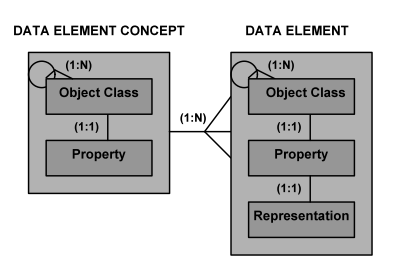
\includegraphics[width=0.6\textwidth,natwidth=610,natheight=642]{figs/DataElementConcept}
\caption{Data Elements and Data Element Concepts} 
\label{fig:DEC}
\end{figure}

The standard continues to describe the relationship between data elements and the concepts associated with them, and also puts forward the notion that a data element is produced when a data element concept is associated with a representation. The notion of \emph{value domains} is introduced, where a value domain is defined as:

\begin{quotation} {sets of permissible values for data} \end{quotation}

  this definition is not very far from the online dictionary of computing definition for the notion of \emph{type}: 
\begin{quotation}
\textbf{type} or \textbf{data type} : A set of values from which a variable, constant, function, or other expression may take its value. A type is a classification of data that tells the compiler or interpreter how the programmer intends to use it. For example, the process and result of adding two variables differs greatly according to whether they are integers, floating point numbers, or strings. 
\end{quotation}

This section then looks in detail at ways in which the conceptual aspects of data elements and value domains are related, and during these discussions the a fundamental model of value domains is presented. Other concepts such as measurement units and enumerations are used to further define the role of the value domain within the standard. Section 1.6 discusses aspects of classification of data elements, apart from the previously introduced notions of object class and property which are part of the Data Element Concept idea. An overview of a metadata registry is introduced in section 1.7, the main feature being that it is a database for metadata built along the lines of the conceptual model provided in section 3 of the standard. Section 1.8 covers the rest of the standard, in addition there is a detailed treatment of terminological principles in the appendix.



\subsubsection{Common understanding of Data}

Part 4 of the standard details how to formulate good data definitions, and data definitions are one of the aspects to achieving a common understanding. The advice in this part of the standard can be summarised as follows: 
\begin{itemize}
\item State the essential meaning of the concept
\item Be precise and unambiguous
\item Be concise
\item Be able to stand alone
\item Be expressed without embedding rationale, functional usage, domain information, or procedural information.
\item Avoid circular reasoning
\item Use the same terminology and consistent logical structure for related definitions
\item Be appropriate for the type of metadata being defined.
\end{itemize}
Use of these guidelines will of course help with the development of a common understanding of data, however it is only when these definitions can be viewed alongside the data item in question that these guidelines can be seen to be useful.


\subsubsection{Re-use and Standardization of Data over time, space and applications}

According to section 5 Standardization involves standardizing the descriptive data itself: characteristics, property values of characteristics, selection of signifiers, and the meaning of values.  It can occur at a variety of levels: agency, national , regional, or international. Governance is further applied by accredited standards organizations, who may well have their own standardization processes. ISO11179-5 details key aspects of naming which should be part of any naming system for data items contained in a registry, and lists a number of criteria which a conforming registry should adhere to. It doesn't prescribe any particular naming system, but rather the key qualities that a naming system should have, and which a registry should document. Part 6 details the organizational requirements for running and administering a metadata registry, however it doesn't specify how re-use or standardization of data over time, space and applications will be enhanced by using an ISO11179 conformant metadata registry. By applying a naming convention to metadata, and by enforcing a rigorous application of that naming convention we can standardise data, however there are no clear practical indications of how this is to be done in the standard.


\subsubsection{Harmonization and Standardization of data}

This is very similar to the purpose of the previous purpose, and again apart from the notes made previously it is difficult to see how the standard itself will further the harmonization of data, apart from the idea of having a uniquely agreed and administered naming and versioning system for data.

\subsubsection{Management of the components \emph{of descriptions} of data}

Here the standard has changed in that the last iteration of the standard has changed the purpose from \emph'{Management of the components of data} to \emph'{Management of the components of descriptions of data}. Most computer scientists would read this as being a change from the idea of \emph{object} to \emph{class}, since an object can be seen as being a component of data, and a class as being a component of a description of data. We consider the term \emph{metadata components} or \emph{models} to be more fitting. Although the management of data components or metadata components is talked about within the standard, it is very often in the terms of the meta-model behind the standard, ideas such as \emph{arranging semantic components with a naming convention} (ISO11179-5.p6) are discussed, but with almost no reference to actual details of what a semantic component is, whether it is referring to combination of a data element and data element concept or an object running in an object oriented programming language. In our view the management models or metadata components is not really addressed by the standard, and it really needs to be.

\subsubsection{Re-use of the components of descriptions of data}

As with the previous discussion we fail to see any direct way in which the standard supports this avowed purpose except indirectly. There is no real definition on what is being referred to by descriptions of data, except in the discussions over what is metadata, when it appears that metadata is defined as being ``'descriptions of data'. This being the case it begs the question of why this purpose is using the terminology \emph{descriptions of data} instead of \emph{metadata}. 




\section{Domain Specific Modelling Language}

\subsection{Language Definition}

\subsection{Semantics}


\subsection{ISO11179}



\section{Metadata Registry}

\subsection{}


\section{Metadata Management}



\section{Results}

\subsection{Comparison of Metadata Registries}


\section{Discussion}

 


\newpage

\bibliographystyle{plain}

\bibliography{md11179}


\end{document}  